\documentclass[10pt,twoside,twocolumn]{article}

\usepackage[bg-none]{dnd/dnd}	%options: bg-a4, bg-letter, bg-full, bg-print; default are bg-letter and bg-full
\usepackage[utf8]{inputenc}

\setcounter{secnumdepth}{5}
\setcounter{tocdepth}{5}

\title{Dunmar: The Dungeon Master's Guide}
\author{Ernest "edg3" Loveland}

% Start document
\begin{document}
\fontfamily{ppl}\selectfont % Set text font

% Content goes after this
\maketitle
\tableofcontents

\section{Introduction}

Welcome to Dunmar, a fantastic city towered over by an even more amazing keep in the mountains of Upcrust. You adventurers are going to be thrown into a world of danger and intrigue that they have not yet explored. Back within the Forgotten Realms a dark terror took control of the entire material plane - your adventurers do not know it but children who have the potential to challenge the rule have been cast into an alternate reality, a man-made plane used to prison enemies of the ideals of one man, this reality where they get to experience the magics of the upper and lower crusts of Renga. \\

Hopefully by the end of this document you will have a clear grasp of the mechanics and special rules that apply to this interesting alternate reality, as well as the broad connections between the tyranny taking place in the Forgotten Realms and the control taking place even inside this world that encompasses the lives of your adventurers.\\

\begin{commentbox}{What is meant by the tyranny in the Forgotten Realms?}
A charismatic drow of very unsubstantial past, named D'quan, in the year of TODO along with a handful of adventurers unlocked a deep dark magic controlling the essence that makes up the planes of existence. D'quan turned against his companions and used the magic to build a new plane of existence, the creation of which released terror and chaos upon the Forgotten Realms
\end{commentbox}

The sections with regards to Early, Mid and Late game are meant as guidelines to give you some idea of how you can have a standard campaign setting. Obviously you can use this setting as you see fit.\\

\subsection{Document Conventions}
Throughout the document you will see boxes of various design being used. \\

% quotebox => descriptive; paperbox => rules/mechanics/examples; commentbox => additional information

\begin{paperbox}{Additional Mechanics}
Boxes like this give additional mechanics, optional rules and/or examples for how to use certain information in this document.
\end{paperbox}

\begin{quotebox}
Boxes like this are generally fluffy information, you can read these out or paraphase them to describe places, people or things to your PCs.
\end{quotebox}

\begin{commentbox}{Informative}
These boxes are used to give additional information on characters and things to you as a DM, either story or mechanics wise.
\end{commentbox}

\subsection{The World}
The world of Renga was created initially as a prison, but the world was too surreal for any inquisitive mind to grasp so the first people exiled to it quickly lost their minds causing them to break out back into the material plane back in the Forgotten Realms. The people were slowly driven to insanity in the empty world and a hidden part of their minds caused them to suffer extreme hallucinations which drove them to reject the reality. The way the plane of existence was created it relied on the deepest darkest hidden parts of the mind to be accepting of the world to stay there.\\

As the original opponents to D'quan's plan began resurfacing in the real world it became clear that more work was needed to make the world habitable by the enemies of D'quan. Through the totalitarian rule of D'quan his opponents were quickly brought before him. Through torture and other extreme interrogation tactics he broke their already twisted minds even further. Incapable of normal cognitive function D'quan realised he could fill his imaginary plane with the memories and ideals of his fallen commrades.\\

Put into a magically induced coma the minds of his former allies (the first returners to the material plane) were cast back into the world and seemingly real beings and nations were born in that plane from their imagination. The people ended up being as real as can be, however if they tried to escape into another plane they would cease to exist as in every other plane they were nothing more than a figment of imagination. The lives of these imaginary people were strong enough to make the world livable for people cast there without losing their sanity, and the world became the perfect prison.\\

Over the last 100 years many hundreds of inhabitants of the Forgotten Realms were cast into this world. Some were prominent politicians, tacticians or magicians. However in the case of your party they may even have been cast to this realm as infants - taken in by the broken minds controlling the world and raised as their own children.\\

\subsubsection{About D'quan and his Party}
D'quan was born a drow inside the material plane. He was abandonned by his family and adopted by a kindly human couple. Despite being brought up as a good being - his life was spent as a reject and was for the most part unwelcome.\\

He left home early and ended up becoming a powerful sorcerer amongst a party of humans, however it did not matter where they went - he was unwelcome and treated badly. He began to hide his appearance and origin as they became stronger as a group and more well known.\\

Eventually the strengths of him and his friends hbegan to rival minor gods and for them to ascend to full godhood they were sent on an almost impossible quest - to find the origin of all magic - in the hopes that they would not succeed. To the dismay of the original gods the party succeeded. Fortunately (or unfotunately) D'quan after learning about the magic for creating planes turned and trapped his party in a plane of his creation, the plane that contains Rengar. He could not further his study of the deep, dark and godly magics without his party's aid but it was a strong enough construct that he used it to banish all people who opposed him in his quest for ultimate power and revenge.\\

Over the years his influence grew and he built armies of people loyal to him - for fear of being exiled to an unknown world. His army marched mindlessly on every corner of the Forgotten Realms and where people opposed his ideals he cast their leaders to Renga.\\

A few years later most of the world was under D'quan's control. The first person to ever return from Renga surfaced, the mind of one of his original companions had broken, and having a broken mind was rejected from the plane. Recognised wondering aimlessly in the material plane the former companion was brought before D'quan. He realised what was happening (from the descriptions put forth by the ancient magic he had used) and worked immediately to rectify it. He ended up casting the first few people that broke down back to his plane. After some time and research D'quan found a way to solve his problem - while the people returning could not function on a high level if he cast them into a magically induced coma they would dream of people and nations in his plane as if it was the proper reality. Delving back into ancient magic he managed to bind their imaginations to his plane and shortly after people stopped being able to break out due to breaking of their minds.\\

He also tasked many sorcerers and architects of strong magic to make the plane as inescapable as possible. While there are still methods to break out of the plane they are rare and difficult to pull off.\\

\subsubsection{The Original Party}
From the original party 3 were cast back into D'quan's realm and 2 became imprisoned in the material plane to harness their imaginations to power the world. The 3 cast back were Obernan the druid-sorcerer, Duvain a warmongering fighter and Barlen a paladin. The two that had their minds enslaved in the material plane were Ren an assassin (who sympathised with the goals of Duvain) and Jene a shapeshifting druid (who was close friends with Barlen) and the world created was influenced primarily by their ideals.\\

\paragraph{The world influence}
Duvain ended up becoming the leader of the movement now called the Varan, simply because Duvain as he regained his sanity believed he was the only person powerful enough to rule this entire world. Barlen who met up with Duvain and recognised him early on Duvain's conquest realised the way Duvain wanted to rule the world was impure and he started a resistance movement called the Iluuminated. Through the years they clashed and eventually an equal ground was found where the two movements were tolerant of one another and what they had achieved. Though Duvain and Barlen did not know it their sympathisers came from the ideals of their captured comrades back in the material planes whose dreams formed nearly the entirety of the living persons whose minds were bound to the people populating this world.\\

\paragraph{The Realisation}
Over time and through the happenings around them people in this realm have an occurence within them called "The Realisation" for Barlen this happened fairly early in the world conquest and he became reluctant to fight with (and have them fight amongst one another) the inhabitants of the world for the fear of damaging the minds of his friends in the material plane further.\\

Duvain on the other hand realised he could raise an army of enemies of D'quan through this world, and ended his fruitless quest for conquest of the land when he realised some of the main footholds of civilization in Renga were too hard to capture (either by their physical locations or strengths bestowed by the imaginations of the minds that controlled the people in those areas).\\

Your PCs may have some inkling from the begining of the campaign that various aspects of the world that make sense are contrasted by things that just dont. As a simple example any sorcerer that focuses on teleportation as their main branch of magic would quickly find that while knowledge of various planes is prominent amongst people (and believed) no supposed method of travel between planes works.\\

It is also important to note that the reason the Illuminated and the Varan still do not join together to form a strong alliance is because while Duvain believes a military strength can fix the material world if they can ever find a way back Barlen instead believes by raising adventurers right and showing them the right paths they will instead find their own ways to opose what is happening in the Forgotten Realms.\\

\paragraph{The Original Party}
The original party will not be explained in detail here since for the entirety of this writing they are either mythical controlling minds or high-up leaders beyond the touch and grasp of the player characters. When the time comes the explanation back in the material plane of their powers and uses will be made clear for when your PCs get out of this prison and are ready to resolve issues back in the real world.\\

Frankly this means if you are only interested in this section of the journey and have your own ideas for after, your own homebrew would exist past the scope of this document.\\

\subsection{Early Game (lvl. 1-7)}
The early game encompasses an important telling of the story of this world and get the player hooked on the world. This can fall into 3 major categories and it is up to you as a DM to decide which of these the characters are veering towards.\\

The 5E factions system lends itself nicely for understanding how a player ends up in a particular track. How the track pans out is up to you, but if you feel you cannot judge accurately you can use the below table:\\

\begin{dndtable}
	\textbf{Action Orientation}  & \textbf{Action Result} \\
   	Illuminated  & The total points acquired for the event added to the Illuminated Total and half removed from the Valar and the full amount removed from the worldly amount \\
   	Valar  & The total points acquired for the event added to the Valar total and half removed from Illuminated and the full amount removed from the Worldly total \\
   	Worldly  & The total points acquired for a worldly happening added to the worldly total and the totla amount removed from each of Illuminated and Valar
\end{dndtable}

As you can see this campaign is highly oriented towards either Illuminated or Valar, but if your PCs instead feel they sympathis with the world itself they would fall under a neutral Worldly banner.\\

The PCs will most likely clash and interact with underlings of the Valar or Illuminated at this stage of this journey and in some places sympathise or ckash with the worldly people.\\

As a DM you will have to steer them to an event that shows the hidden conflict and power struggle between both groups and let them decide for themselves which group they will end up joining. The decision does not need to be explicit since if they gain favour with a specific group that group will reward them.\\

\subsubsection{Illuminated}
Being Illuminated means the characters have built a strong belief that whomever resides in the world should be in control of what happens to them. This means their recruits are volunteers and straying from their path is forgivable if it falls inside the beliefs of the Illuminated.\\

The Illuminated want only to restore the power in the Forgotten Realms to where they were before D'quan took complete control with no reparation or revenge, only a restoration of balance.\\

\subsubsection{Valar}
The Valar are clearly bent on revenge, and the militaristic ideals of Duvain mean that essentially they will be building an army with strict control with a distinct purpose of forcefully taking control of the Forgotten Realms from D'quan.\\

The Valar want to take back control in a manner that they feel they are rightfully owed, and as such are willing to go to any extreme to overthrow D'quan and his illusions.\\

\subsubsection{Hermits}
Obernan of the original party opted not to take part in the squabbles of his fellow party members, he took to the wilderness and began to attune himself to the nature of this world as he did not want to disturb the people that formed the minds and imaginations of his comrades back in the material plane who populated this world. Not completely sane his travels led him to many secrets of the world, and while he avoided people he became somewhat of a legend amongst the imaginary people as he would turn up in times of dire need and save people and dissapear without a trace shortly after.\\

\begin{commentbox}{Obernan the Worldly}
Obernan falls squarely in the category of "worldly" oriented beings. He has a deep disgust for both the way of the Valar and the Illuminated. When his path crosses the adventurers if they are doing good according to the worldly people there will be no issue, but if major Valar or Illuminated ideals are shown they will have a tough time dealing with him. He is willing to thrash anyone opposing him within in inches of their life but will not kill unless he absolutely has to.
\end{commentbox}

The other hermit in this land is Replin, he was not part of the original party but was one of the people that got cast into the world once D'quan had fixed the problems with containing people in the world. He was part of the original group that helped D'quan make it impossible to leave Renga, he does have some offhand knowledge of the gates and how to activate them but was never privy to locations of all the parts, he did however come in posession of one of the Gate keysshortly after Krent left his service. He is hesitant to tell people about his origin and the source of his magics, due to the strength of the magic stopping cross-plane teleportation he has resigned himself to the fact that he is trapped in this world.\\

\subsubsection{Worldly}
The worldly tract will be the hardest to judge for your players. The death of D'quan will lead to the destruction of the plane and this will have untold consequences on all other existing planes, however without stopping D'quan many more people throughout time will be destroyed, including the "imaginary" people of this plane of existance.\\

Players on the worldly tract will have to abstain from the beliefs of the Illuminated and the Valar but rather be more involved in the greater good. The worldly tract focuses on the desire to make the plane permanent and save everyone, while despite the good or bad intentions of a faction ultimately the party will realise the dillema from either outcome being the downfall of the people they have come to know.\\

\subsection{Mid-game (lv. 8-12)}
By now your players should have been introduced to a lot about the world and have some idea of how they can escape the world (see "Escaping Mechanics") and likely even be well on their way to breaking out from the world. In this part there will likely be clashes and assaults involving the generals of the opposition movement and a sort-of "arms race" to be the group that breaks out first.\\

Your PCs will likely be in the thick of things and in the middle of the chaos as their strength has grown and they should be able to tip the balance between the Valar and the Illuminated. You will need to guide them and their needs to come to the end of this arc of their story where they find a way back to the material plane (see "Escaping Mechanics").\\

Note that if the PCs are oriented against Valar or Illuminated (or both) the forces will be actively seeking to thwart their plans as they want to be the ones to break out of Falr and take control of the plane. It is clear that from the Valar side they want to simply take forceful control of the magic controlling the plane and destroy it whereas the Illuminated want to convinced D'quan to destory the plane, or convince him to relinquish control of it.\\

\subsection{Late-game (lv. 12+)}
Late-game assumes you have broken into the material plane and have goals to do with D'quan.\\

TODO: add in mechanics and enemies and plot elements for the material plane.

\section{The Guilds}
Understandably the Valar and Illuminated are not actuall guilds, however they effectively function like a guild would.\\

\subsection{The Valar}
As you should surmise the head of the Valar is Duvain an expert in melee combat who prefers to use a broadsword for combat. His influence of control is managed by 3 generals one in control of each city in his sphere of influence.\\

\subsubsection{The Generals}
Duvain's 3 generals have extremely different spheres of influence, but they make up a formiddable team willing to get their hands dirty fighting for the goals of Duvain. They are level 12 characters (see appendix A) who are not meant to be trifled with by players till near the end of the course of this module.\\

The first general is Krent, a halfling sorcerer who has a taste for destructive magic. He is ruthless but fair, not hesitating to punish someone who doesn't do right by him, but strong enough that people don't dare challenge him. He first met Duvain in the forest of Darkwood, they had both been there for different self-illuminating reasons and had made the mistake of lighting a fire incurring the wrath of the Treants that resided there - both barely escaped with their lives after working together and a strong bond was formed between them.\\

\begin{commentbox}{About Krent}
Krent is an outspoken person with a sharp tongue and a love for harsh language. Krent was cast into this world as a baby and taken care of by Replin the hermit sorcerer who brought him up. Krent grew to love fierce magic and was eventually cast out by Replin to wander the world as his taste for destruction grew too much. At a young age he joined a militaristic group and quickly rose in power. After a few years of fighting he became tired of it and decided he wanted to go on a self-exploratory journey through the world, and when his journey took him into Darkwood this is where he met Duvain and found out about his origins. His hatred for the ideals that D'quan forced upon Krent and other material plane beings drove Krent to join Duvain.
\end{commentbox}

The second general is Femble a pale skinned lady with jet-black hair. Very little is known about her other than she has never lost a duel and she carries no weapons. Rumour has it she has in her past come across Strahd himself and been given extraodinary power by him. During Duvain's second major campaign aginst what he thought was a completely imaginary kingdom after storming the strongholds of Kvoth it is rumoured that Femble had killed a group of 12 of Duvain's best fighters. Duvain had then challenged Femble to a 1v1 battle and the battle lasted 2 days, after which Femble swore loyalty to Duvain.\\

\begin{commentbox}{About Femble}
Femble is the quietest of Duvain's generals, she is soft-spoken and doesn't often reveal much of her personal details. She is well-aware of the turmoil back in the material plane as that was where she grew up. How she was cast to this plane was actually not of D'quan's doing, but rather in her quests she ended up in the Underdark and her journey took her directly to Strahd. Strahd placed a curse on her granting her something akin to immortality as long as she drank the blood of willing persons daily and when she finally got a Wish to escape the material plane she chose to exile herself to this world of Renga. As she became accustomed to this world she realsied that many people in it needed saving from the magic of D'quan and she joined with Duvain as he was the first that came before her in this world.\\

At Femble's side at all times is her closest companion in the world Jeni, the people closest to Femble know they became close friends early on when Femble ended up in this world and Jeni offered herself willingly for Femble to feed on as long as she lived. Many people have speculated that they are lovers too, but that is the sort of thing that Femble does not share with people, people do however know she would do anything to protect Jeni and if any harm were to come of Jeni it was certain Femble would unleash her full wrath on whomever was stupid enough to do so.
\end{commentbox}

The third general is Teekim a gnome tinkerer who managed to build himself amazing mechanical and magical constructs and he rules his domain with machines rather than recruits. Shortly after coming into the world Teekim had realised the strength of his power in this plane and having heard of Duvain's goals he built up an army of constructs and stormed Duvain's personal quarters as a show of power - not to harm Duvain, but to recruit himself to Duvain's cause - impressed by the willingness to fight and the sheer strength of the constructs Duvain welcomed Teekim to his army as a general.\\

\subsection{The Illuminated}
The illuminated have a rather different structure. Barlen himself has himself as one of the 3 leaders of the Illuminated, his 3 main generals he made friends with and hold them as equals. Two of which form the main leadership of the Illuminated and the last forms their general strategiser.\\

\subsubsection{The Generals}
The first general is an elf by the name of Brittlebow a paladin herself. In the early days when most chaos and bloodhsed occured in this imaginary world many worldly people were attacked in the power struggle between the Valar and the Illuminated. After learning the ideals of the Illuminated were more towards her own ideals she built up a company and got people to infiltrate the ranks of the Valar - using information gained to cut-off attacks on the worldly people with her company. Barlen caught wind of this and approached Brittlebow to be an ally and an equal. Eventually the city of ??? asked for the Illuminated to control their affairs and Barlen placed Brittlebow at its head.\\

The second general is a being of unknown origin, known only as the Seer. The Seer had an odd habit of appearing at a place of battle and turning the tide in the favour of the Illuminated and then dissapearing without a trace, clad from head-to-toe in a red cloth no features of the Seer were distinguishable, and hence nobody knew who it was. Somehow the Seer was captured by the Illuminated and convinced by Barlen to join the forces officially, his identity and power is still unknown to this day.\\

\begin{comment}{More on the Seer}
The Seer is actually a child of D'quan himself by the name of Dartaun, a drow that was raised in the material plane. His appearance is hidden for the fact that he is a splitting image of his father. He stood up against his father when he found out what was happening to his father's enemies and got himself cast into the imaginary world. His specialty magic is a magic he developed himself allowing to corrode the armor and dull the blades of the enemies that face him. He also maintains a special magic nullification field that causes magic missiles cast at him to be repelled straight back at the sender.
\end{comment}

The third general is an extremely socially inept elvish druid by the name of Mossdeepner, his foresight was able to see that without a strategic direction the sheer brute force of the Valar would quickly overrun the world and push their ideals on the people. He brought himself to Barlen and proposed he should control the strategy of the Illuminated, he managed to convince Barlen it was the best course of action and has lead the forces of the Illuminated since. Being at the age of 343 he avoids combat but has a deep experience and knowledge that he uses to outwit and outsmart his enemies. Due to his age his mind does slip at times and is often found in a state half transformed into a bear (who coincedentally has grey fur and a long beard). Though he does avoid fights he is a formiddable opponent and has been known to knock strong opponents unconscious with ease without even being in his bear form.\\

\subsection{The conflict}
The conflict between the two groups over the last 100 years was a clear show of force with the Valar blatantly attacking cities with armies to take control of them. The Illuminated instead took control of cities by saving them from forces of the Valar and good relations. The cities that have stood as neutral ground have either been insignificant in the greater scheme of things or heavy strongholds that are very difficult to assault (for example Dunmar is surrounded by treacherous mountains which are hard to bring large armies over).\\

\begin{paperbox}{Plot Hook}
A good way to introduce a player to this realm and story is to bring them to a neutral city, such as Dunmar, and have them become invited to the splendour of such a magical place. Slowly draw them into the subterfuge between the Valar and the Illuminated.\\

This technique is used in the podcast which was used to reveal and build this setting at the start. The adventurers finally arrive in Dunmar towards the end of their last day of travel and were taken to a cozy inn on one of the main roads. In the middle of the night they are woken by strange noises outside to find dark robed figures running about incapacitating guards in a non-lethal manner. The party jumps out and tries to stop them to find out they are Illuminated out on a mission to recover a stolen artifact.\\
\end{paperbox}

\section{Cities, Towers and Towns}

The cities each have their own rules and specific management, you can obvious forgo a lot of this information and just refer back if you need additional inspiration. \\

\subsection{Alcomby}
\textbf{Alignment:} Good \\
\textbf{Faction Orientation:} Worldly \\
\begin{quotebox}
	Alcomby is a small settlement where roughly 2000 people live, it is on the Northern edge of the continental lake on Upcrust. The building are very simply wood and stone houses you would find in a typical fishing town and they have a port that has ships coming in and going out from daily.\\

	The people are very laid back and simple, welcoming to strangers. Their primary incomes are from selling fish caught in the lake to neighbouring areas and ferrying people across the lake when people don't want to take the long detour around it. The settlement is managed by a Sheriff and his 6 deputies who have 100 or so men under them doing all the grunt work, as such they are spread pretty thin and theft is a real problem here.\\

	There are many fishmongers and bars along the lake-front, various shops that sell general items and specialty items for ships and fishing. You would be hard-pressed to find a magic shop or dealer, and if you do they would like be of ill-repute. Other professions (e.g. smithing, etc) are available but there are only a few places you could go for such services. Most of the inns are also in the lake-front, many built ontop of the various bars.
\end{quotebox}

\subsection{Aston}
\textbf{Alignment:} Good \\
\textbf{Faction Orientation:} Illuminated\\
\begin{quotebox}
	Aston is a settlement on the Southern edge of the continental lake on Upcrust, housing roughly 8000 people it is a bustling business zone where many people deal in traded goods. They have a bustling market from fish but their primary money comes from trading items bought from the Clockwork City's large industries.\\

	The people here are very friendly and do not take kindly to trouble-makers. The guard is vast and strong and make their presence known, though while it is a very lawful town they often have large street parties and festivals throughout the year - courtesy of the vast amounts of barley farming on the outskirts of Aston feeding a network of dwarven breweries.\\

	You can find most kinds of shops and services here, however magically enchanted items are extremely expensive as they are mostly magical constructs of the Clockwork City. There is a legend that there is a black market masquerading as a gentleman's club - however the only gentleman's club in the settlement has been investigated often and nothing indicates they run a black market.
\end{quotebox}

\subsection{Aurilon}
\textbf{Alignment:} Good \\
\textbf{Faction Orientation:} Worldly \\
\begin{quotebox}
	Aurilon is a secluded keep on one of the outer Upcrust mountaintops. There is a single way to get into Aurilon, rarely the airship will drop off supplies and bring back people that want to leave the place and taking people that want to go there. The airship drop point is a good 2 day hike from the peak where the actual keep is. The keep stands atop the mountain and is built of iron, steel and huge blocks of ironstone - that the mountain is made of.\\

	The people here are very reserved and very strong, high level mages and paladins look after the keep itself, they do not make friends with strangers often as most visitors there are there to head into the dungeon the keep covers the entrance of a horrific dungeon below.\\

	There are no shops and services available here. When you get here the only thing offered to adventurers is a process to allow them into the dungeon for the price of 1000gp per person which is a process involving writing your will and wishes for storage at the keep and after paying you then may enter as many times as you want. The caveat being there is no guarantee you can find your way back.\\
\end{quotebox}

As a side note, the dungeon below Aurilon is a weak rift between this plane of existence and all others. While it is widely accepted by both Valar and Illuminated that there must be a way through it back into the material plane - countless parties have enterred and either never returned or have had only one or two members return in a state that they cannot communicate what happened in there with other people, broken men and women. \\

\subsection{Aysgarth}
\textbf{Alignment:} Evil \\
\textbf{Faction Orientation:} None \\
\begin{quotebox}
	A lone tower on Undercrust the monolithic tower extends all the way from the depths of Downcrust up to the island holding Wealdstone. It has large glowing runes all around the outside and only a single entrance at the bottom. The tower is so large that you can see it from the airship when travelling to and from Wealdstone. \\

	Originally it is believed the tower was built to hold up Wealdstone as parts of landmass connecting it to the rest of Upcrust not much is known about it other than the location to the entrance to it from Upcrust isn't common knowledge and people are ushered away by the city guard of Wealdstone if they happen to find it.\\
\end{quotebox}

Aysgarth has been taken over by Ice Mephit, Yetis and the cries of a dragon have been heard by those who have ventured inside before.

\section{Special Mechanics}

\subsection{Travel Between Planes}
Travel into the Dunmar plane (where this world exists) from any other plane of existence requires only that have either been to the plane yourself or you have an attuned rod to the plane. Traveling out of the Dunmar plane is impossible other than from the mechanics in the section below "Escaping Mechanics", that is any traditional method for moving off a plane of existence will appear to fail with no reason.\\

\section{Escaping Mechanics}
One of the main driving factors for your PCs will be to escape the plane (whatever their personal preference of ending will be) to do this there are several special mechanics.\\

\subsection{Using a Gate}
The gates will be the safest mechanic for a player to escape the world, they require a few artifacts scattered around the world:\\

\begin{itemize}
\item A Gate key (either obtained as an heirloom or retrieved inside Dunmar)
\item Gate attunement crystals (these are used to power a gate and scattered across the world, these rare stones are depleted after use)
\end{itemize}

Once a gate is found with a gate key and an attunement crystal the players will need to power the gate up with a crystal and first defeat the horrors and aberrations such a "dirty" gate would unleash into the world (when powering the gate up since it is not a normal plane of existence it draws in inter-dimensional beings to attack the party).\\

Once the "guardians" of the gate are defeated the PCs can all stand in the area of the Gate, turn the key and be teleported to the corresponding gate in the real world. It is important to note that the corresponding real world locations are in control of D'quan as he uses the gates to send his enemies into the world, the keys and attunement crystals were hidden should he accidentally be cast into his own world and need to escape.\\

\subsection{The Underdark}
The Underdark is a special exception to the plane travelling rules of this world. It may come to be that your PCs cannot get what they need to power up a gate and escape through it, then it may be clear that they have to find a way into the Underdark - a place of horridble creatures and high danger.\\

The gates into the Underdark grow in places that light never touches, as such this will require your players to take a perilous journey onto the lower crust and into the mines and catacombs beneath the lower cities. Since the lower crust is built from the dark thoughts and secrets of the imaginations running the world the cities are full of murderous and dangeroud beings that live in a chaotic manner.\\

Once in the Underdark the PCs will need to find a being capable of helping them escape back to the material plane (through any standard means of getting from the Underdark to the material plane).\\

\section{Things that can leave this plane}
As was mentioned earlier any imaginary being of the plane cannot exist outside of that plane of existence. However all physical items and beings can leave the plane.\\

The justification for this is that the beings while imaginary had a physical manifestation and special magic about them within the plane, their influence on the world therefore was as physical as it was imaginary. Should the minds be unplugged from the plane of existence all the imaginary beings would dissapear but their physical changes to the world (cities, belongings, etc) would stay as they were made of physical objects.\\

\subsection{Optional Mechanic: Constructs}
As an optional mechanic you can use a magical method of binding a soul to a physical construct and that would allow the soul to survive leaving the world. Essentially this says that when a character dies their soul gets stuck in this plane.\\

\begin{paperbox}{Constructs Example}
A PC dies on a quest - you can allow the PCs if they are friends with Teekim to get a construct built for the dead player and get Krent to bind the soul to the construct. You can homebrew this as necessary yourself - or base it on existing homebrew (5E Warforged, see Appendix D).
\end{paperbox}

\section{Random Encounter Tables}

\subsection{Using the Tables}
When players are heading to a city for some reason at your discretion you should roll for a set of events for the city, there are a handful of rolls available and are split into sections of their own.\\

\begin{paperbox}{Example of Encounter Generation}
The PCs are heading to Dunmar, as they are approaching you first roll for "Overarching Story Feature", we get a 2 indicating an Illuminated Encounter.\\

We roll for Illuminated Encounters getting a 1 launching "Rescue by Night" - meaning on one of the nights in this city the Illuminated are sending a party to try save some of their captured comrades.\\

As an Illuminated party some member of the Illuminated might come ask the PCs to help and it would be a stealth mission. As a Valar oriented party the PCs would hear scuffles happening outside wherever they are staying and upon investigation try and stop the Illuminated from their goals.
\end{paperbox}

Note that these are to supplement encounters with the correct story hooks for the world, and are meant as guidelines for setting up the events. As such there is no way to know what level your PCs will be, however broad mechanics and information will be given so you can give your players an appropriate challenge.\\

Also note that you can give information of future events to drive story as you see fit. At the end of the quest above you might roll an event for Mournstead and get a Valar attack will happen occur there, driving the players to start a journey to Mournstead - similarly possibly causing you to use another encounter to open up one of the easier pathways to Downcrust.\\

\subsection{Overarching Story Feature}
Roll 1d4 to select one of the following:\\

\begin{dndtable}
	\textbf{Dice}  & \textbf{Result} \\
   	1 & Valar Encounter \\
	2 & Illuminated Encounter \\
	3 & Fabric of Plane \\
	4 & Worldly Encounter \\
\end{dndtable}

Additional note, if a 3 is rolled reroll if not for one of Butterpond, Wellspring, Wealdstone or Grimsby.\\

\subsection{Valar Encounters}
TODO: Valar Encounters\\

\subsection{Illuminated Encounters}
Roll 1dX to select one of the following:\\

\begin{dndtable}
	\textbf{Dice}  & \textbf{Result} \\
   	1 & Rescue by Night \\
\end{dndtable}

\subsubsection{Rescue by Night}
If the players are Illuminated oriented they may be contacted by an Illuminated member to fill them in on the details, otherwise players might be woken in the middle of the night by a commotion outside.\\

A party led by Illuminated underlings has gotten information that a bar in a bad part of the city has been used as a base of operations for the Valar and a friend of theirs is being held there, they are on a rescue mission. To avoid the harm of worldly people and attracting the attention of the guard they are using Knock Out Needles (see Ap. B) and when they find a person that comes from the material plane using these needles they will switch to using more force.\\

Running this event will be a medium difficulty skill check initially, with the outcomes being:\\

\begin{dndtable}
	\textbf{Faction}  & \textbf{Goal} \\
   	Valar & Slow or stop the advance of they Illuminated without getting attention of the city guard \\
	Illuminated & Stay stealthy and try to get to the bar before the guard discovers the party \\
	Other & You will need to discern if they PCs choose how they want to proceed how you will run the check,
\end{dndtable}

\section{Alternate Skill Checks}
You can use any method that works for running a skill check for encounters in this setting, however we offer this suggestion of how to run them for this setting:
PCs will roll initiative to work out their turn order, on their turn they will describe what they do and how they will use their stats to support their action. You will decide a suitable DC (see "DC Tables" below if you need help) or opposing roll (for example if an action is taken directly against a character) and you need to decide if the action counts as a fail outright, an alternative setback or a pass.\\

Additionally you make it so that players cannot use the same stat as the person before them, or the stat that they used on their previous turn.\\

\begin{paperbox}{Example}
In a chase where players need to stop (without killing) a suspect fleeing from a crime scene, it is a simple chase of Easy difficulty. Following from partly through the chase (towards the end):\\

\textbf{DM:} Alright player 1, what is your action?\\
\textbf{P1:} Do I see any guards in the direction he is running away?\\
\textbf{DM:} Yes, there are several guards but they aren't taking action.\\
\textbf{P1:} Ok, I roll charisma to shout at them, "Hey, stop that thief!" - rolling a 17 charisma check.\\

You decide it is an appropriate action, the PCs have been here for a while helping the king it is likely some guards will recognise the party and set the DC at 50\% for his +5 charisma (DC16) - he passes.\\

\textbf{DM:} Two of the guards take into action and start trying to cut off the thief, that is a Pass. Player 2, you may go.\\
\textbf{P2:} I do my best to chase after him and try close the gap to him, I want to use my intelligence to try and use a simlpler path than he is running.\\
\textbf{DM:} Unfortunately so far he is just running in a straight line away from you, but you could use dexterity instead and try beat his speed?\\
\textbf{P2:} Sure, I roll a 7 for dexterity.\\

You will choose that being an easy action its an 80\% chance with his +5 to dexterity meaning his DC was 10, meaning he failed.\\

\textbf{DM:} You stumble and slow down the party members behind you and thus earn a Fail in the chase. Player 3, your turn.\\
\textbf{P3:} Ok, I cant use dexterity, my next best stat is strength. What do I see around me?\\
\textbf{DM:} You are essentially in a marketplace, there are various tables laid out with wares around you, mostly freshly set up, there are only the stand owners around and guards since it is still early in the morning.\\
\textbf{P3:} How far would you say we are from the assailant?\\
\textbf{DM:} Probably about 8 or 9 squares (45ft roughly).\\
\textbf{P3:} Ok, I am going to go with crazy here, I want to pick up and try throw P1 (a dwarf) towards the assailant if that is fine with Player 1?\\
\textbf{P1:} Sure.\\
'textbf{P3:} I roll a 22 for strength.\\

You set the DC as quite difficult (25\% chance vs his +7 to strength) making the DC 22.\\

\textbf{DM:} You are successful and P1 lands just behind the assailant taking 1d4 damage from the throw, that is a Pass, one more pass needed. Player 1, back to you, this action will have advantage as the guards will make him slow a bit and check for trying to change direction as he is close to running into them.\\
\textbf{P1:} Ok, I guess I should use dexterity here as I want to uncoil my rope and throw a loop around the assailant while running to catch him, that would be a 14 and 21, so 21.\\
\textbf{DM:} How would you say you want to try wrap the rope around him?\\
\textbf{P1} I basically grab 2 parts like a skipping rope and try throw it over his head.\\

You decide this is a reasonably simple action and set it at 65\% chance for his +5 dex meaning the DC was 13.\\

\textbf{DM:} You successfully throw the rope over him and grind to a halt effectively clotheslining him and he slams down into the ground, that is a Pass. Skill check over.\\

\end{paperbox}

\section{Appendix A: Character Sheets}
TODO: Duvain [lv.15 human fighter]

TODO: Barlen [lv. 15 human ???]

TODO: Krent [lv. 12 halfling sorcerer]

TODO: Femble [lv.12 human assassin/vampyr ~ note: impervious to sun]

TODO: Teekim [lv. 12 gnome tinkerer/sorcerer]

TODO: Fighter of Krent [lv. ??? fighter]

TODO: Sorcerer of Krent [lv. ??? sorcerer]

TODO: Underling Fighter of Krent [lv. ??? fighter]

TODO: Underling Sorcerer of Krent [lv. ??? sorcerer]

TODO: Assassin of Femble [lv. ??? assassin]

TODO: Underling of Femble [lv. ??? assassin/ranger]

TODO: Major construct of Teekim [lv. ??? magical construct]

TODO: Minor construct of Teekim [lv. ??? magical construct]

TODO: Seeker of Teekim [lv. 1 magical construct ~ note: used for hunting specific people down, little hovering robots]

TODO: Brittlebow [lv. 12 paladin]

TODO: The Seer [lv. 12 drow sorcerer]

TODO: Mossdeeper [lv. 12 elvish druid of bear]

TODO: Knights of Brittlebow [lv. ??? fighters]

TODO: Squires of Brittlebow [lv. ??? fighters]

TODO: Agent of The Seer [lv. ??? Assassin/sorcerer]

TODO: Hand of The Seer [lv. ??? thief]

TODO: War bear of Mossdeeper [lv. ??? bear]

TODO: War hound of Mossdeeper [lv. ??? hound]

\clearpage

\section{Appendix B: Items}

\begin{itembox}{Knock Out Needle}
	\textit{A small non-lethal poisoned needle.}\\
	\hline \\[1mm]
	\begin{itemaction}[Action: Jab]
		Jab a character with a neede to try knock them out.\\
		Roll a dexterity check +5 to hit versus AC:\\
		Hit on wordly character: the character is instantly knocked out.\\
		Hit on PC or unworldly character: the character becomes drowsy and actions are taken at a disadvantage for 5 minutes
	\end{itemaction}
\end{itembox}

TODO: Gate Key

TODO: Gate Attunement Crystals

\clearpage

\section{Appendix C: Plot locations}

\subsection{Upcrust}

Travel: 1 hex is 1 week fast travel to across (i.e. on horseback with a hard push during the day), closer to 2 weeks with slower relaxed travel. \\

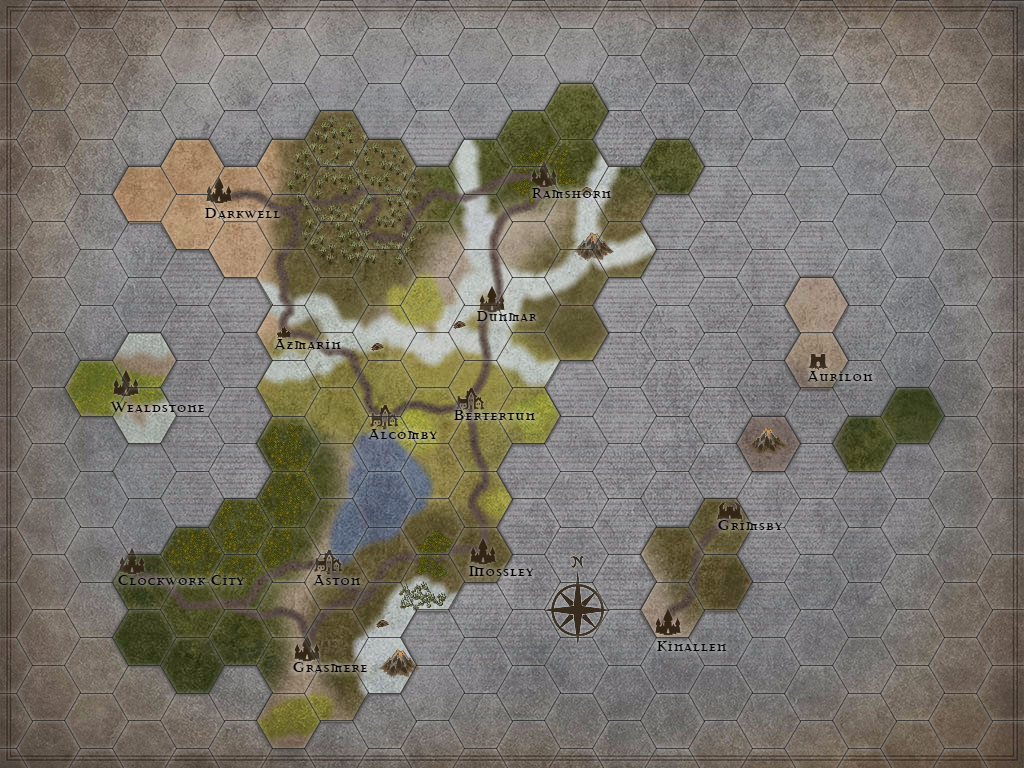
\includegraphics[width=\textwidth]{Images/Maps/Upcrust}

\clearpage

\subsection{Downcrust}

Travel: 1 hex is 1 week fast travel to across (i.e. on horseback with a hard push during the day), closer to 2 weeks with slower relaxed travel. \\

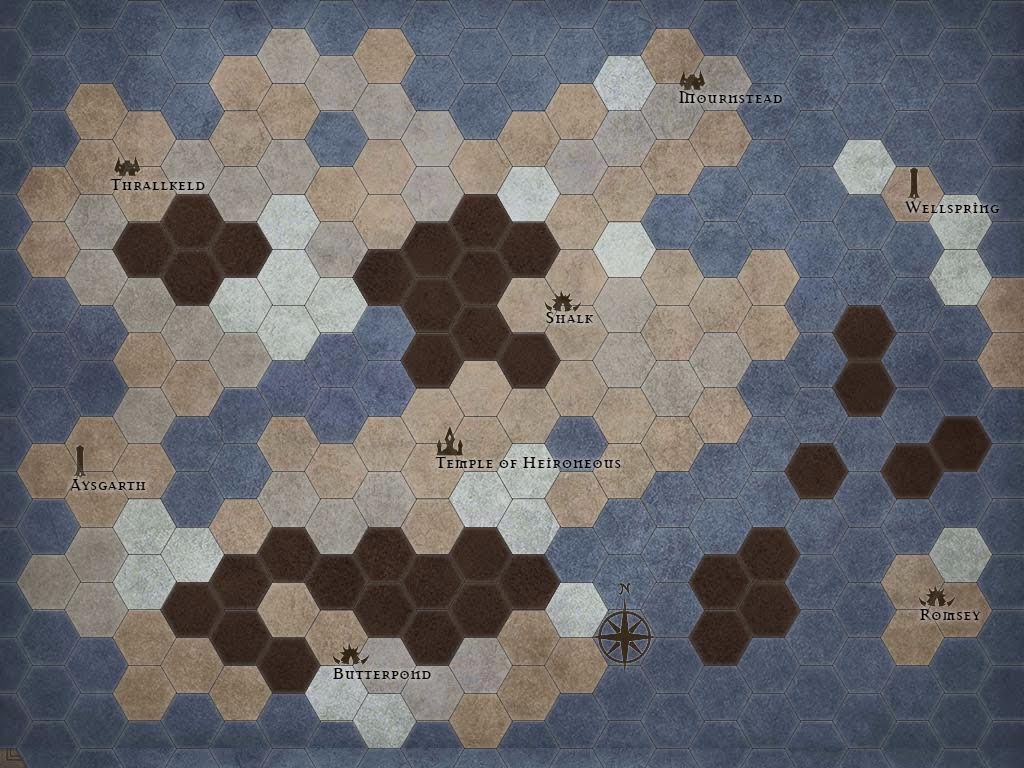
\includegraphics[width=\textwidth]{Images/Maps/Downcrust}

\clearpage

TODO: Maps of cities

TODO: Maps of castles

TODO: Maps of the 3 gate locations

\section{Appendix D: Useful Resources}

\begin{itemize}
\item Map Building - http://inkarnate.com/
\item 5E Warforged - https://www.dandwiki.com/wiki/Warforged\_(5e\_Race)
\end{itemize}

% End Document
\end{document}
